% !TEX root = main.tex
\chapter{Understanding the current paradigm for certificate issuance }
\label{chap:Understanding domain validation practices}

% ==============Introductory Remarks====================== %

\section{Introductory Remarks}\label{sec:chap3Intro} 

HTTPS plays an important role in the maintenance of user privacy when communications take place on the web. Using HTTPS, Internet users can communicate with a web service in a privacy-preserving manner --- \ie the communication channel is private from any other entity that may be privy to the communication channel (\eg ISPs, mobile carriers, back-bone servers, company/organization gateways \etc ). However, the compelling guarantees provided by HTTPS rely on a trust model that includes certificate authorities (CAs). Excessive trust that is being placed on these authorities has led them to act as single point of failures --- a single malicious or compromised CA can enable HTTPS connections to be vulnerable to eavesdropping, message modification, or injection of malicious scripts. The following issues illustrate the root of the PKI problems on the web. 

\paragraph{The number of CAs has exploded.} In order to accomplish the trust in a CA based PKI, software companies \eg Microsoft, Mozilla, Apple, and Opera place a default whitelist of self-signed CA certificates in the firmware of an embedded system and/or browsers as trusted root certificates. Therefore, while visiting an HTTPS website, the browsers merely accept those sites certificates whose validity has been attested by at least one of the trusted root certificates in that whitelist. For instance, Microsoft Windows includes ${\sim}$350 trust anchors from ${\sim}$140 companies. Trusted root CAs can also issue certificates that authorize other organizations to act as a CA. Thus, the actual number of trusted CAs is greater. Later in this chapter, we show that about 223 companies are browser-accepted.

%The SSL Observatory reports that between Microsoft's Internet Explorer and Mozilla's Firefox, ${\sim}$1500 CA certificates from ${\sim}$650 organizations in ${\sim}$50 countries are browser-accepted \cite{eckersley2010observatory}. We will 

\paragraph{CAs are targets for privacy breaches.} Each trusted CA can issue a browser-acceptable certificate for any site. Hence, an adversary can deceive a weak CA to obtain a fraudulent certificate for a domain he does not own (\ie \texttt{adversary.com}). By doing so, he is able to actively intercept every single communication that takes place between the server hosting \texttt{adversary.com} domain and other entities on the web. For example, In 2011, malicious parties were successfully able to illegitimately obtain certificates from the two significant CAs --- Comodo \cite{eckersley2010observatory}\cite{ComodoRe52:online} and DigiNotar \cite{kaminskypki}.

There is also increasing concern that some CAs are vulnerable to certificate compulsion attacks. In this type of attacks, governmental entities force CAs to help them with surveillance by issuing fraudulent certificates for specific website to be spoofed, which they can then use to intercept and tap individuals' secure HTTPS connections to those websites \cite{soghoian2011certified}. Surveillance can occur in private networks as well \eg in enterprises where computers are operated by employers. In this case, organizations can install a root CA certificate on employees' machines which allows them to perform MITM attacks and intercept any HTTPS communication that is established from those computers. Some client-side software, such as anti-virus and parental control, also use a MITM attack to inspect HTTPS content and this can leave the end user vulnerable depending on subtle configuration issues \cite{de2016killed}. 

\paragraph{We know very little about CAs.} Although some research has been carried out on HTTPS ecosystem, our knowledge in the full spectrum of CAs is still very limited. What is not yet clear is the number of CAs that actually issue certificates to the public. Additionally, certification practice statements (CPSs), the only techniques that are used by CAs to validate the ownership of domains during the issuance of certificates, are reported to be poor. These techniques have been developed and established by CAs based on their practical experience over a few decades and there is no consensus about the mechanisms that are used by every CA for domain ownership validation.

The purpose of this chapter is to assess and examine real-world CAs on their domain validation practices while issuing certificates. Our first objective is to develop a full enumeration of all uniquely identified trusted CAs that can be traced to a real world entity and issue certificates to external websites referred as \emph{companies} in our work. As a second goal, we attempt to formulate a detailed documentation of the existing validation mechanisms undertaken by companies. The scope of our documentation includes the domain validation techniques performed by companies~\cite{Alternat16:online}, potential vulnerabilities (\eg if documented parsing errors can be exploited \cite{BlackHat94:online}), personal information that companies collect during a domain validation process, and the costs related to issuing certificates to the public.

\paragraph{The Invisibility of Intermediate CAs.} There are two categories of certificate authorities: (i) explicitly trusted root certificate authorities that are recognized by root certificates. These self-signed certificates play a significant role in establishing trust in PKI, they are transmitted to end users by secure physical distribution \ie being preinstalled on devices. (ii) Implicitly trusted intermediate or subsidiary certificate authorities that have been delegated with the certificate issuing power from root or already-authorized intermediate CAs. There is no solid record of intermediate certificates that currently exist on the web. This is because intermediate certificates can be issued by a root certificate authority (delegating certificate issuing power to another CAs by signing their certificates and creating a certificate `chain') and this authorization is unknown by anyone until a certificate chain is observed in the wild that uses the intermediate CA. As a result, there is no way to establish how many companies have been issued an intermediate CA. The best we can do within today's PKI is observe as many certificate chains as possible---\eg by scanning the entire internet or logging certificate chains from consenting users as they browse the web.

% =====================Methodology================================ %
\section{Establishing the Number of Authoritative Entities}

To evaluate certificate authorities (CAs) and domain ownership validation procedures they employ, we first need to identify these third parties. These authorities consist of root certificate authorities and intermediate (or subsidiary) certificate authorities. We use other research projects that have measured the internet to enumerate the current list of intermediate certificates that have been seen in the wild. Our analysis begins with collecting a complete record of (i) root and (ii) intermediate certificate authorities:

\noindent\textbf{Root Certificate Authorities.} As explained earlier, software vendors such as Microsoft, Mozilla, Apple, and Opera configure extensive lists of built-in root certificates in operating systems and/or browsers, by doing so, they securely transmit the root certificates to the end users. In order to collect the root certificate authorities, between April and June 2015, we retrieved the list of root certificates from (i) Microsoft Windows, (ii) Apple OS X (including OS X Yosemite, iOS 7, iOS 8, Watch OS), and (iii) Mozilla Firefox. After merging these data and collapsing multiple identities for the same CAs, we developed a shortlist of ${\sim}$259 actual unique root certificate authorities called \emph{Condensed Root CAs} which we believe is the most comprehensive record of all the current root CAs. 

\noindent\textbf{Intermediate Certificate Authorities.} Data related to the intermediate certificate authorities on the entire web was collected using the major research projects that have been conducted in the CA ecosystem. (i) We used the data provided by the SSL observatory, an EFF project that investigates the SSL certificates on the Internet \cite{eckersley2010observatory}. (ii) We employed the data supplied by three projects \cite{durumeric2013analysis}\cite{SSLCerti90:online}\cite{MoreSSLC62:online} that use the ZMap \cite{haldermanfast}, an Internet scanner tool to widely scan and analyze the HTTPS environment. (ii) Lastly, we used known certificate logs from Google's certificate transparency, which provides a monitoring and auditing framework for SSL certificates by appending valid certificates to these logs \cite{laurie2013certificate}. The data collected from these project was then parsed and processed and eventually merged into the list called \textit{Intermediate CAs} which contains a list of ${\sim}$446 actual unique intermediate certificate authorities.

% =====================Analysis And Results================================ %
\subsection{Analysis and Results}

There has been little quantitative analysis of how many of the current certificate authorities (including root and intermediate) are actually unique organizations that provide certificate issuing services to the public. Thus, to gain insight into the domain validation procedures, we first require to identify those CAs who directly provide certificates to the end users, considering the fact that some CAs only issue certificates internally or are managed by a different CA. To do so, we manually research the ${\sim}$700 intermediate and root certificate authorities that were gathered in the data collection procedures. By visiting these CAs websites, it was found that merely ${\sim}$223 of these \emph{companies} actually issue certificate to users. Having the list of the companies developed, the final section of this analysis undertakes domain control validation (DCV) methods, deployed by each of these parties. To achieve this for each company, we chose to obtain a regular one year single-domain certificate for a domain name we control. Clearly, we only targeted domain validated (DV) certificates because we did not possess a registered organization nor were we able to be verified in person (to obtain organization validated (OV) and extended validated (EV) certificates). Using the DV certificate purchases as a pilot, we developed a comprehensive enumeration of the companies such as (i) the number of companies that actually issue SSL certificates (EV,OV,DV) to a member of the public, (ii) the cost of acquiring certificates, (iii) the country where each company is located, (iv) contact information of companies, (v) information to be provided to CAs during the domain ownership verification, (vi) how this information is used and (viii) how is identity of users validated.

% =====================Results================================ %

In the first stage of our scan, we contact each company in the list to obtain a certificate for our domain, we discover that only 71 of these companies actually issue at least one of the EV, OV, DV certificates to the public users. The other 152 companies cannot provide certificates to us due to the following reasons:
\begin{itemize}
\item They only issue certificates to their own country services \eg universities and research institutes.
\item They only issue certificates to services from the national government agencies.
\item They only issue certificates in projects.
\item They only issue certificates to the external partners/vendors that do business with their company.
\item They require a face-to-face registration for any type of web server certificates. This is either at their office,or via a notary in applicant’s country.
\end{itemize}

Therefore, we complete our survey by contacting 71 companies that assuredly provide certification services to us (as a public user from a foreign country). The results of our survey indicate that among 71 companies, 42 of them are willing to issue domain validated (DV) certificates to end users (see Figure ~\ref{fig:VennDiagram}). 

% =====================Venn diagram Figure================================ %
\begin{figure}
\begin{center}
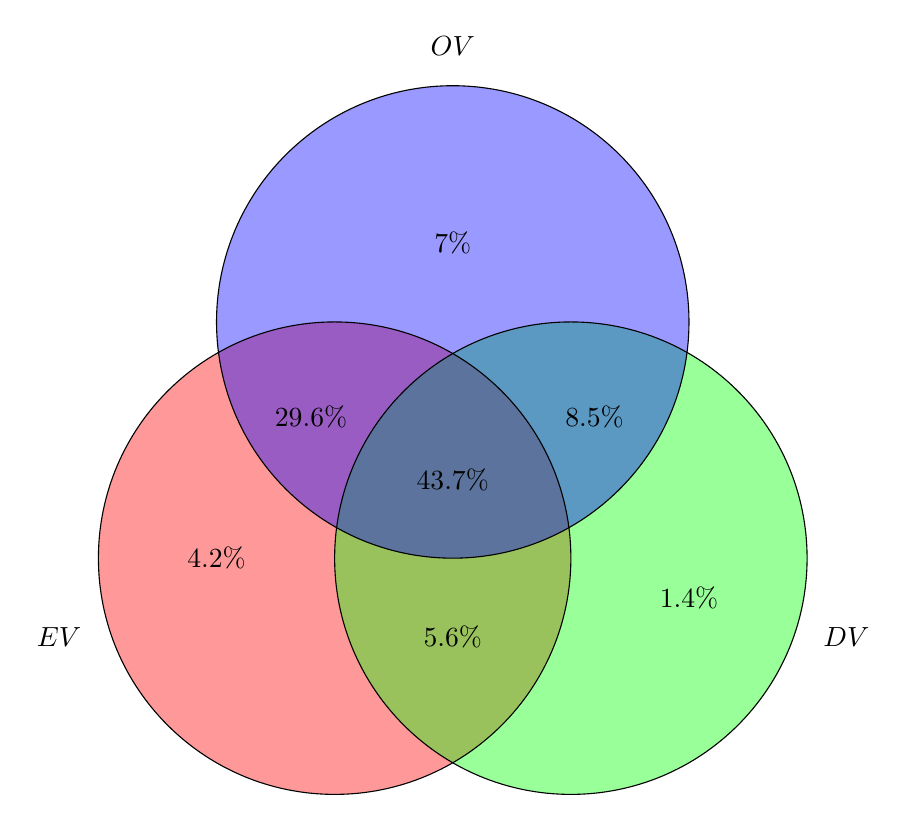
\begin{tikzpicture}
[fill opacity = .4, text opacity=1]

\fill[red] (0,0) circle (3cm);
\fill[green] (3,0) circle (3cm);
\fill[blue] (1.5,3) circle (3cm);
\draw (0,0) circle (3cm);
\draw (3,0) circle (3cm);
\draw (1.5,3) circle (3cm);
%________________________________________________%
% \draw (-1.5,0) node {\textbf{$EV Only$}};
% \draw (-1.5,-0.5) node {$4.2\%$};
\draw (-3.5,-1) node {\textbf{$EV$}};
\draw (-1.5,0) node {$4.2\%$};
%________________________________________________%
% \draw (4.5,0) node {\textbf{$DV Only$}};
% \draw (4.5,-0.5) node {$1.4\%$};
\draw (6.5,-1) node {\textbf{$DV$}};
\draw (4.5,-0.5) node {$1.4\%$};
%________________________________________________%
% \draw (1.5,4.5) node {\textbf{$OV Only$}};
% \draw (1.5,4) node {$7\%$};
\draw (1.5,6.5) node {\textbf{$OV$}};
\draw (1.5,4) node {$7\%$};
%________________________________________________%
%\draw (1.5,-1) node {\textbf{$EV \& DV$}};
\draw (1.5,-1) node {$5.6\%$};
%________________________________________________%
%\draw (-0.3,2.3) node {\textbf{$EV \& OV$}};
\draw (-0.3,1.8) node {$29.6\%$};
%________________________________________________%
%\draw (3.3,2.3) node {\textbf{$DV \& OV$}};
\draw (3.3,1.8) node {$8.5\%$};
%________________________________________________%
%\draw (1.5,1) node {\footnotesize{EV \& DV \& OV}};
\draw (1.5,1) node {$43.7\%$};
%________________________________________________%
\end{tikzpicture}
\end{center}
\caption[Distribution of the certificates issued by 71 companies]{Distribution of the certificates issued by 71 companies --- We found that a large group of these companies only issue the high assurance (OV and EV) certificates.}
\label{fig:VennDiagram}
\end{figure}
% ====================================================== %

Furthermore, results reveal that 73.3\% of these companies issue extended validated (EV) and organization validated (OV) certificates, which are both considered as high assurance certificates. The reason behind this is, as explained earlier, due to the existing drawbacks in domain control validation (DCV) procedures that allow malicious parties to obtain fraudulent certificates for domains they do not control. By acquiring a fake certificate for victims domains, adversaries can perform MITM attacks and intercept traffics before victims can receive it. This is while DV certificates are often preferred above all other certificates because (i) they are offered at much lower prices than high assurance (EV and OV) certificates and (ii) they are issued during effortless and automated processes. We also found that 33.3\% of the companies that issue DV certificates are currently located in the United States. 

After reviewing each company's certificate practice statements (CPS), we discovered the companies do not always document their certificate issuance policies in a precise manner. In some cases, verification procedures that companies provide in their CPSs are not equivalent to what they offer in practice.

% =====================Threat Modeling (Is it really a good term?!)===========================%
\section{Showcasing the Indirection Used by CAs}

Domain control validation (DCV) procedures are a set of techniques employed by certificate authorities to verify the ownership of a (sub)domain that certificate is asked for. Unlike high assurance certificates, domain validated (DV) certificates only represent a certificate holder's control over a given domain name and they do not provide any intuition about the identity of the owner. DCV can be performed using any one of the (i) email-based, (ii) HTTP-based, and (iii) DNS-based methods. What follows is a brief description of the DCV methods and the security issues with them.

% ================Email Based Validation===================================%

\paragraph{Email-based Validation.}

Email-based validation is the most supported method of host name verification. In this approach, CA sends a unique nonce as a secret challenge to an email address it is assumed to belong to the subscriber. If the certificate applicant can access this challenge, it is considered to have proven ownership of the domain and causes the CA to issue the certificate. CAs specify a list of acceptable addresses for a given domain using a few generic names including \texttt{admin}, \texttt{administrator}, \texttt{hostmaster}, \texttt{postmaster}, and \texttt{webmaster}, in addition to any email addresses that appears on a domain's WHOIS record. 

% ================HTTP Based Validation===================================%
\paragraph{HTTP-based Validation.}

In this technique, the CA delivers a unique, non-secret nonce (or hash of the certificate request) to the subscriber through an HTTPS channel. In order to prove domain name ownership, the subscriber needs to create a text file with the nonce and upload the file to the root directory of his domain that is to be validated. In the final part of the verification process, CA checks the presence of the text file. If the file is successfully retrieved by the CA and its contents match, domain control is confirmed.

% ================DNS Based Validation===================================% 
\paragraph{DNS-based Validation.}

Using the DNS based method, the subscriber receives a unique, non-secret nonce (or hash of the certificate request) from CA through an HTTPS channel and he is required to publicize the nonce in his DNS CNAME record for the domain. Afterward, the CA queries the corresponding name servers to verify the presence of the DNS CNAME record. If the record is successfully obtained, domain ownership is validated.

% ================Indirection and Authoritative Issue===================================% 

\subsection{Authoritative Issue}

 In the current web certificate model, certificate authorities are meant to be $authorities$: that is, they are authoritative over the namespace they bind keys to. The reality is that the web still runs largely on domain validated certificates~\cite{DKBH13}\cite{HBKC11} and for domain validation, certificate authorities generally are not any more or less authoritative over who owns what domain than you or I. There is arguably no single party that is authoritative. ICANN manages the top-level domains and delegate registration of domains to registrars. Registrars sell domains to companies or individuals. Registrars do not identify the people buying the domains; instead they have the purchaser set a username/password for an account that they can use to manage the domain. Registrars are natural entities to serve the role of a CA and indeed there is overlap between the set of registrars and the set of CAs, however a registrar/CA is not restricted to issuing certificates to only its own customers and can in fact issue certificates for any domain. Many CAs are not registrars or connected in any way to the domain management eco-system. They establish who owns a domain through indirection.
 
\subsection{Indirection Issue}\label{indirection} 

\begin{figure}[t]
\centering
\includegraphics[width=0.9\textwidth]{Fig/attacksonDCV.png}
\caption{\footnotesize{Possible attacks on the DCV techniques.}}
\label{fig:attacksonDCV}
\end{figure}

% JC: change website to HTTPS. Add reserved email to email subtree. 

A central problem with the certificate model is that CAs resort to \textit{indirection} to issue certificates because they are not directly authoritative over who owns what domain. For example, email based DCV involves 2 levels of indirection: (1) CAs appeal to DNS to establish the MX record of the domain (\ie the subscriber's mail server'��s IP address); and (2) CAs appeal to SMTP to establish a communication channel to the subscriber. For every level of indirection, there are a set of vulnerabilities which might allow a malicious party to break the verification process and obtain a fraudulent certificate for a domain they do not own.

To illustrate this in more detail, we will consider email-based validation as described above. We note that email validation works in conjunction with DNS, so the vulnerabilities on this process subsume the set of vulnerabilities of DNS-based validation. We leave aside HTTP-based validation as it is largely similar; but we note one interesting issue: the CA must fetch the posted hash of the certificate request from the website and since the website is trying to obtain a certificate, it follows that they likely do not have an existing certificate and therefore are not providing this file over HTTPS. Any man-in-the-middle between the webserver and the CA could respond to the CA's request with a fraudulent CSR (even if it doesn't actually exist on the webserver) and obtain a fraudulent certificate. 

We now enumerate at list of threats to email-based validation to illustrate how broad the attack surface becomes when excessive indirection is relied on. These are summarized in Figure~\ref{fig:attacksonDCV}.

\begin{enumerate}

\item \textbf{Reserved Emails:} A CA specifies a list of email addresses to receive the challenge. The underlying assumption is that only the domain owner controls this address. However the domain owner might not reserve that email address or even be aware that a certain email address is being used by one of the CAs for this purpose. And recall that just a single CA needs to use a single non-standard email address (\eg a translation of administrator into their local language) to open up this vulnerability. For example, Microsoft's public webmail service \texttt{login.live.com} saw an attacker successfully validate his ownership of the domain using an email address \texttt{sslcertificates@live.com} which was open to public registration~\cite{zusman2009criminal}.

\item \textbf{Whois Emails:} A CA will also optionally draw the email address from the Whois record for the domain. A domain's whois record is generally protected by the username/password set by the domain owner with their registrar. Any attack on this password (\eg guessing or resetting) or directly on the account (\eg social engineering~\cite{GoDaddyo45:online}) would allow the adversary to specify an email address that they control. 

\item \textbf{MX Record:} A CA will establish the IP address of the mailserver from the MX record for the domain. As above, all domain records including the MX record is managed through the owner's account with her domain registrar. Any method for obtaining unauthorized access to this account would enable an adversary to list their own server in the MX record and receive the email from the CA.

\item \textbf{DNS Records:} If an adversary cannot directly change a DNS record, they might conduct other attacks on the CA's view of DNS. For example, they might employ DNS cache poisoning which can result in invalid DNS resolution~\cite{son2010hitchhiker}. They might also exploit an available dangling DNS record (Dare)~\cite{liu2016all}.  A Dare occurs when data in a DNS record (such as CNAME, A, or MX) becomes invalid but is not removed by the domain owner. For example, if the domain owner forgets to remove the MX record (the IP address of the server) from DNS, the associated DNS MX record is said to be dangling. If an adversary can acquire this IP address at some future point, he is able to redirect all traffic intended for the original domain to his server, including information sufficient for a CA's domain validation process. Thus a malicious party can use a Dare to obtain a fraudulent certificate.

\item \textbf{SMTP:} Once the CA establishes the mailserver's record, it will send the email to the mailserver with SMTP (the standard protocol for transfer of email). Since the email contains a secret nonce, confidentiality of this email is crucial. SMTP uses opportunistic encryption that is not secure against an active adversary. Thus a man-in-the-middle between the CA's mailserver and the ultimate destination (including an forwarding mailservers) could request a fraudulent certificate, intercept the ensuing email, reply with the correct nonce, and be issued the fraud\-ulent certificate.

\item \textbf{Email Accounts:} Email accounts are generally protected with a username and password (over IMAP or POP3) to prevent unauthorized access. In some cases, they might be protected with a client certificate. An adversary who can gain access to any one of the accounts that should be reserved by the domain owner (\eg texttt{admin}, \texttt{hostmaster}, \texttt{webmaster}, \etc) could obtain a fraudulent certificate for that site. This could include guessing or resetting the password, using social engineering, or obtaining access to the server hosting the email for the account. 

\end{enumerate} 

% ================Conclusion===================================% 

\section{Conclusion}

In this chapter, we developed a complete enumeration of all the existing certificate authorities. We then surveyed the procedures these CAs enforce in order to validate domain name ownership during the certificate issuing processes. It has been discovered that while domain validation methods seem promising, they are not completely secure in practice and can be compromised by malicious parties on the web. As a result, attackers are able to deceive and/or compromise the CAs to sign invalid certificates on behalf of them. We also discussed the major issue with the the current certification system is that the entities that issue a certificates for domain names (CAs) are not the actual domain's owners. We believe that certificate authorities are not special and any entity that owns a domain can be a CA and issue a certificate for that domain. In fact, Verisign is not more authoritative than anyone else in the case of validating domain names. 

As discussed above, these third parties (CAs) are vulnerable to a vast group of vulnerabilities that if compromised, an adversary obtains a certificate for a domain that does not belong to him. This issue can be addressed by designing a system in which the domain owner can issue and manage certificates without having to rely on any third party. By removing the CAs from this infrastructure and make entities authoritative over their domain names and certificates, we can eliminate single point of failures and their prominent consequences from the public key infrastructure. 

In the next chapter, we introduce our system which is a new paradigm for the certification model. Using this new system, we will be able to eliminate certain limitations of the current CA model. As it was discussed in Section~\ref{sec:chap3Intro}, currently a large number of CAs (${\sim}$300) exist on the web and this is while the root CAs can still delegate their issuing certificate power to the other CAs. However, our proposed scheme eliminates the 300 CAs and replaces it with \emph{one} decentralized, authoritative system. Further, the system is fully authoritative over domain names and cryptographic keys and so no indirection is necessary. 


